\documentclass[11pt, oneside]{article}   	% use "amsart" instead of "article" for AMSLaTeX format

\usepackage{PopDyn}
\externaldocument{PopDyn_Appendix}
\title{Population Dynamics of Socially Learning Predators}
\author{Talia Borofsky}
%\date{}							% Activate to display a given date or no date

\begin{document}
\maketitle
\section{Introduction}
Learning by foragers can have profound effects on their foraging niches and hence the population dynamics of the organisms in these niches \cite{gil2018social}. Many animals, especially but not exclusively vertebrates, can learn from conspecifics how to forage \cite{galef2001social, giraldeau2018social}. Socially acquired information about a forager's food environment can influence its preference for certain food types or foraging patches \cite{galef2001social, slagsvold2011social} and this preference can persist over long timespans, even for an animal's entire life \cite{slagsvold2011social}. Thus social learning may result in between-generation associations that limit plasticity in response to resource depletion or environmental change \cite{gil2018social}. 

It is unclear which environments select for social learning and how social learning by foragers affects their own population dynamics and those of the resources they use. When food becomes more limited, foragers may benefit by augmenting their diet with food items that are less utilized by others \cite{giraldeau1984group,aljadeff2020competitive}, a phenomenon called the skill pool effect \cite{giraldeau1984group}. For example, although house sparrows can learn socially, in an experiment in which na\"ive sparrows watched trained  conspecifics foraging, the (formerly) na\"ive sparrows tended to use different food cues to locate food from those used by their demonstrators, all of which used a single cue \cite{aljadeff2020competitive}. In fact, groups of sparrows that used a mix of cues performed better at finding food than those that all used the same cue. In a previous evolutionary one-consumer, two-resource model with a static environment and constant consumer population size \cite{borofsky2021conformity}, social learning was less adaptive as resources became more limited because social learners tended to harvest one resource more intensely than the other; social learning prevented the skill pool effect. Social learning had the same effect in an agent-based model with a changing environment \cite{smolla2015competition}. However, if social learning was payoff-biased and individual learners could not learn about how to forage on more than one type of resource at a time, then social learning was adaptive irrespective of the level of competition for resources \cite{borofsky2021payoff}.

Thus social learning may lead to very different population dynamics from those where foragers only use individual learning to find food. Previous models have shown that social learning by prey about predators (as opposed to social learning by predators, the focus of this paper), such as potential prey overhearing and reacting to each others' alarm calls, decreased the amplitude of fluctuations in predator and prey population sizes \cite{toth2021hidden}. Learning by predators may also lead to stable persistence of prey populations if the learning causes predators to focus on harvesting more common food types \cite{van2001alternative, ishii2012learning}. However, unbiased social learning, which entails that social learners adopt a behavior randomly from the demonstrators they watch, causes foragers to have diet preferences that may not be concordant with the actual quantities of food types available. We thus expect that unbiased social learning by predators, as opposed to individual learning, will destabilize equilibria where both prey types and the predator coexist, causing either fluctuating population dynamics or extinction of one of the prey types.

In this paper, we investigate the feedback between population dynamics and the evolution of social learning by predators. We construct a one predator, two-prey model and ask the following questions:
\begin{enumerate}[start=1, label={(Q\arabic*)}]
\item Can social learning cause a predator population to drive a prey population to extinction?
\item Does social learning increase predator population size?
\item Do conditions under which social learning evolves depend on whether the predator population size is constant or changing?
\end{enumerate}

In our previous models \cite{borofsky2021conformity, borofsky2021payoff} there was a time delay in the dynamics of the prey (or resource): the amount of resources available by the end of the current generation was a function of predation by adults from the previous generation rather than by adults in the current generation. In this model, we examine whether our answers to the above questions depend on whether there is a time delay.

%\item When two prey types are available, generalist predators without a strong preference for either disproportionately attack the more common prey species \cite{murdoch1969switching, murdoch1975switching, ishii2012learning}. In parasitoids this pattern has been attributed to the development of search images \cite{ishii2010effect, ishii2012learning}, where a search image is a preference for searching for a specific prey type that results in the predator ignoring or not detecting other prey types \cite{ishii2010effect}. 


%Previous studies have examined predator-prey dynamics when the predators cooperate. How cooperation alters dynamics in a one predator-one prey model was addressed in \cite{berec2010impacts}, and the dynamics in a one-predator, two-prey system in which predators cooperate and the two prey populations have a mutualistic relationship in \cite{banerjee2020cooperative}. Social learning can be thought of as a form of cooperation, but there are two main differences between models of social learning and cooperation. Social learning is often vertical, where information is passed from parents to offspring, or oblique, where offspring learn from the parental generation, although not necessarily from their parents \cite{cavalli1981cultural}. Therefore models with vertical or oblique social learning may require a time delay. Furthermore, role models can exhibit different behaviors and a social learner has to choose which demonstrated behavior to adopt. Thus a model of social learning should track the number of individuals exhibiting the various behaviors. 




%We present a one predator, two prey model based on the Rosenzweig-Macarthur predator-prey model (\cite{rosenzweig1963graphical} as described in \cite{turchin2003complex}), in which we incorporate social learning. Our questions are:
%\begin{enumerate}
%\item As food becomes more limited, does increasing the probability of social learning decrease or increase equilibrium predator population size? More specifically, as the prey birth rate decreases relative to the predator's maximum kill rate, does increased social learning cause a decrease in the equilibrium biomass of the predator population?
%\item How does the inclusion of individual and social learning affect population dynamics of predators and prey in relation to models without social learning?
%\item Apparent competition has been observed in other one-predator two-prey models in which predation intensity increases (nonlinearly) with the prey's population size \cite{van2001alternative}. Does apparent competition emerge when there is only individual learning? And how is this affected by social learning?
%\end{enumerate}
\section{The Model}

We construct a one-predator, two-prey system which can also be thought of as a one-consumer, two-resource system. In any generation, predators are born, they learn from the previous generation's food preferences, and their survival to adulthood is determined by their success at finding food. The predator population size is $N_p$. To make the analysis more tractable, as in \cite{van2001alternative}, we assume that one of the prey types has a constant population size.  The prey type with a changing population size will be called the changing prey (CP) and has population size $N_r$, carrying capacity $C_r$, and density relative to its carrying capacity, or frequency, $r = N_r/C_r$. This prey type will be called the alternate prey (AP) and has a fixed population size which we assume is less than the carrying capacity of the CP, $N_R < C_r$. Let the normalized density of the alternative prey be $R = N_R/C_r$ (normalizing in this way allows $r$ and $R$ to have the same scales).We assume that the prey populations do not compete with each other. Different predator behaviors are required to capture the different types of prey with the behavior to capture AP (hereafter referred to as the AP behavior) being innate whereas individuals must learn the behavior to capture CP (the CP behavior). At any time, predators exhibit either the AP behavior or the CP behavior but not both. 

The model assumes haploid genetics where we take $\mathbf{B}$ to be a social learning locus with alleles $B$ and $b$ denoting the resident and mutant alleles, respectively. The resident type learns socially with probability $K$ whereas the mutant type learns with increased or decreased probability $K + \dk$. The frequencies of predators of type $B$ that hunt AP and CP are $u_R$. and $u_r$, respectively. The frequencies of predators of type $b$ that hunt AP and CP are $x_R$. and $x_r$, respectively. The frequency of predators with alleles $B$ and $b$ are $u=u_R + u_r$ and $x = x_R + x_r$, respectively, where $x = 1 - u$.  

As in \cite{henrich1998evolution, wakano2007social, borofsky2021conformity, borofsky2021payoff}, foragers interpret information in their environment about how to find food, which may be accurate, difficult to interpret, or inaccurate. The quality of information is represented by $z$. If $z > 0$, then information is accurate, and as $z$ increases, information about how to find food is easier for the forager to interpret. If $z < 0$, then the information is inaccurate, and the more negative the value of $z$, the more inaccurate the information. If foragers are able to learn socially, then we assume they tend to learn socially if information is ambiguous and difficult to interpret, i.e. $z$ is close to $0$. We assume that the information quality in the environment $z$ has a Gaussian probability density function $f(z)$ with mean $\mu$ and standard deviation $\sigma = 1$. The probability that (a) predators individually learn a successful foraging behavior, i.e. learning the correct behavior to hunt the CP, (b) predators socially lear a foraging behavior, and (c) predators use individual learning but adopt an unsuccessful foraging behavior, are
\begin{subequations} \label{learningprobs}
\begin{align}
\pc &= \int_s^\infty f(z) dz \\
K &= \int_{-s}^s f(z) dz \\
\pw &= \int_{-\infty}^{-s} f(z) dz,
\end{align}
\end{subequations}
respectively, where $s$ is the social learning cutoff. Carriers of allele $B$ have social learning cut-off $s$ and learning probabilities $\pc$, $K$, and $\pw$. Carriers of the mutant allele $b$ have social learning cut-off $s + \ds$ and learning probabilities $\pc + \dpc, K + \dk,$ and $\pw + \delta_{\pi_W}$ which result from substituting $s + \ds$ for $s$ in Eqs. \ref{learningprobs} a - c. Note that $\dpc + \dk + \delta_{\pi_W} = 0$.
The probability that a carrier of allele $B$ adopts behavior CP is assumed to be
\begin{equation} \label{L_u}
L_u(p_r,r) = Kp_r + \frac{r}{r+R} \pc,
\end{equation}
where $p_r = u_r + x_r$ is the total frequency of individuals hunting CP, the term $K p_r$ is the frequency of adopting behavior CP from unbiased social learning, and $\frac{r}{r + R} \pc$ is the probability that a predator adopts behavior $CP$ by individual learning. The probability that a carrier of allele $B$ adopts behavior $AP$ is $1 - L_u(p_r,r)$. The probability that mutant $b$ adopts behavior CP is
\begin{equation} \label{L_x}
L_x(p_r,r) = (K + \dk) p_r + \frac{r}{r + R} (\pc + \dpc) = L_u(p_r,r) + \dk p_r + \dpc \frac{r}{r+R},
\end{equation}
and the probability that a carrier of $b$ adopts behavior $AP$ is $1 - L_x(p_r,r)$.

The life history of predators is divided into juvenile and adult stages. After birth, juveniles learn how to find food at rates
\begin{subequations} \label{rec_juveniles}
\begin{align}
\tilde{u}_r &= u L_u(p_r,r) \\
\tilde{u}_R &= u (1 - L_u(p_r,r)) \\
\tilde{x}_r &= x L_x(p_r,r) \\
\tilde{x}_R &= x (1 - L_x(p_r,r)).
\end{align}
\end{subequations}

Juveniles consume food then pass to the adult stage. The frequencies of individuals surviving to adulthood and exhibiting behaviors CP and AP are $u_r'$ and $u_R'$, respectively, if they carry $B$, and $x_r'$ and $x_R'$, respectively, if they carry $b$. Consuming food provides a survival fitness increment, which is $r$ for the CP and $R$ for the AP, so the survival fitnesses of those that learn how to hunt the CP and AP are $1 + r$ and $1 +R$, respectively, and these are frequency-dependent because $r$ and $R$ can be thought of as frequencies. The recursions are
\begin{subequations} \label{recursions}
\begin{align}
W u_r' &= \tilde{u}_r (1 + r) = u L_u(p_r,r) (1+r)\\
W u_R' &= \tilde{u}_R (1 + R) = u(1 - L_u(p_r,r))(1 + R)\\
Wx_r' &= \tilde{x}_r(1+r)  = xL_x(p_r,r)(1+r)\\
Wx_R' &= \tilde{x}_R(1+R) = x(1 - L_x(p_r,r))(1 + R),
\end{align}
\end{subequations}
where $W$, the mean population fitness, is the sum of the right sides of Eqns. \eqref{recursions}, namely,

\begin{equation} \label{eq_W_all}
W= 1 + R + (r - R) \lrb{ L_u(p_r,r)+ x \lrp{ \dk p_r + \dpc \frac{r}{r+R}} },
\end{equation}
as shown in Appendix \ref{Derive_W}.

The population size $N_p$ of the predators, once they reach the adult stage, is
\begin{equation} \label{rec_N_p}
N_p' = N_p \lrp{W - \delta}, 
\end{equation}
where $\delta$ is the death rate of predators. 

For the dynamics of the resource (prey) populations, we study two models: one in which resources are depleted and learning occurs at the same time (no time delay), and one in which resource depletion occurs before the new generation learns how to find food (the time delay model). 
%\red{I'm not sure how to reduce the number of parameters for the prey equations below. It would help if the predator population had some sort of 'maximum' size, e.g. if at a certain density predators somehow interfere with each other beyond competing for food. This could look like
%\begin{equation}
%N_p' = \frac{N_p(1 - \delta + W)}{1 + cN_p}
%\end{equation}
%for $c$ a constant determining density-dependence, which is loosely based off of \cite{din2013dynamics}. Then $\hN_p = \frac{W - d}{c}$
%} 

The prey population in the current generation is depleted by predation, expressed as the term $N_p P(r, u_r, x_r)$, where the rate of predation on the CP, $0 \leq P(r,u_r,x_r)\leq 1$, will be defined later. Similarly to \cite{borofsky2021conformity, din2013dynamics, asmussen1977density, roughgarden1979theory}, the population size of CP after foragers reach adulthood is
\begin{equation} \label{N_t}
N_r' = \frac{N_r(e - f N_p P(r, u_r,x_r)) }{c + d N_r},
\end{equation}
where  $e, f, c$, and $d$ are nonnegative constants. The constant $d$ controls density dependence, $e - c$ determines population growth, and $f$ is the effect of predation. If there is no predation on the $CP$, i.e. $f N_p P(r,u_r,x_r) = 0$, then the steady state population size of the CP, $\hat{N_r}$, is at its maximum $\hat{N_r} = C_r = \frac{e-c}{d}$, assuming $e > c$. We assume $e > c$ and thus $r = \frac{N_r d }{e-c}$. Then substituting into \eqref{N_t}, we have
\begin{equation}
r' = \frac{r(e-f N_p P(r,u_r,x_r))}{c + r(e-c)}.
\end{equation}
Let $\eta = \frac{e}{c} - 1$ be the CP density growth constant and let $\beta = \frac{f}{c}$ be the rate of prey depletion by predators. Then
\begin{equation} \label{r_recursion}
r' = \frac{r(1 + \eta - \beta N_p P(r,u_r,x_r))}{1 + r \eta}.
\end{equation}
The equilibrium frequency of the CP is $\hr$, and $\hr = 0$ or the solution to
\begin{equation} \label{r_hat_general}
r = 1 - \frac{\beta}{\eta}N_p P(r, u_r, x_r).
\end{equation}
Since $0 \leq P\lrp{\hr,\hu_r,\hat{x}_r} \leq 1$ and $0 < \hr \leq 1$, we must have $N_p < \eta/\beta$. To reduce the number of parameters, assume $\eta = 1$.

\subsection{No time delay}
The prey population in the current generation is depleted as the juvenile predators survive to adulthood.  Then 
\begin{equation}\label{L_total}
P(r,u_r,x_r) = L_{total} = u L_u(p_r,r) + x L_x(p_r,r)
\end{equation}
is the total frequency of adult foragers hunting for the CP in the current generation. \red{Equation \eqref{r_hat_general} is not enough to solve for $\hr$.}

\subsection{Time delay}
Here, prey in the current generation are depleted by adult predators from the previous generation. The rate of predation on CP is $P(r,u_r,x_r) = p_r$, recalling that $p_r = u_r + x_r$. Hence, the equilibrium density is $\hr = 0$ or 
\begin{equation} \label{r_hat_delay}
\hr = 1 - \beta \hN_p \hat{p}_r.
\end{equation}


\section{Results}
\subsection{Existence of equilibria with mutant allele $b$ absent}
Here all predators are of type $B$ and we investigate the equilibrium properties of the system \eqref{recursions}, \eqref{eq_W_all}, \eqref{rec_N_p}, and  \eqref{r_recursion} if there is no time delay, i.e. the predation term is defined in \eqref{L_total}, or if there is a time delay, i.e. the predation term is $p_r$. In the absence of $b$, this system becomes
\begin{subequations} \label{sys_allB}
\begin{align}
N_p'&= N_p(W - \delta) \\
W u_r' &= L_u(u_r,r)(1+r),
\end{align}
\end{subequations}
where
\begin{equation} \label{W_allB}
W = 1 + R + (r-R) L_u(u_r,r).
\end{equation}
The prey recursion is
\begin{equation} \label{r_allB}
r' = \frac{r (2 - \beta N_p P(r,u_r))}{1+r},
\end{equation}
where $P(r,u_r) = P(r,u_r,0)$.

The following results apply to the model without a time delay, for which the predation term is \eqref{L_total}, and to the model with a time delay, where the predation term is $p_r = u_r$:

\begin{lemma} \label{Result_L_delta}
If $\hN_p > 0$ at equilibrium and $R \neq \hr$, then
\begin{equation} \label{delta_eq}
L_u(\hu_r,\hr) = \frac{\delta-R}{\hr-R}.
\end{equation}
\end{lemma}
\begin{proof}
From Eq. (\ref{sys_allB}a), at equilibrium $\hw = 1 + \delta$ if $\hN_p > 0$. Then from \eqref{W_allB},
\begin{equation}\label{before_delta_eq}
\delta - R = (r-R) L_u(u_r,r)
\end{equation}
which simplifies to \eqref{delta_eq}. Thus the equilibrium learning rate depends on predator death rate and the prey frequencies of CP and AP.
% which is valid if $\hr \leq \delta < R$ or $R < \delta \leq \hr$.
\end{proof}
%and since $0 \leq L_u(\hu_r,\hr) \leq 1$, $\delta \leq \hr \leq 1$. \red{Should this be in methods (the part where I describe the model) since this puts a limit on a constant?)}

\begin{lemma} \label{Order_R_delta_r}
If there exists $\hN_p > 0$ then  one of the following is true for the equilibrium values of $\hr$ and $\hu_r$:
\begin{enumerate}[(i)]
\item If $R = \delta$ then $\hr = R$ or $K \hu_r = \hr = 0$. 
\item $\hr \leq \delta < R$
\item $R < \delta \leq \hr$.
\end{enumerate}
\end{lemma}
\begin{proof}
The proof is in Appendix \ref{Proof_Order_R_delta_r}.


\end{proof}


\begin{lemma}\label{Result_eq_Rlessthandelta}
If $R < \delta$, then there is one nonzero $\hu_r, \hr, \hN_p$ equilibrium if $\beta > 0$ and
\begin{equation} \label{exists_eq_Rlessthan}
\pc(1-R) + (\delta-R)(1+R) \lrp{ \frac{2K}{1+\delta} -1 } >0.
\end{equation}
\end{lemma}
This inequality is depicted in Fig \ref{fig:result3_1}. %\red{WHAT HAPPENS IN THE UNSTABLE REGIONS?}
\begin{proof}
The proof is in Appendix \ref{Proof_eq_Rlessthandelta}. 
\end{proof}
In Appendix \ref{Proof_eq_Rlessthandelta}, we show that under the conditions in which $\hr > 0$ exists, $\hr$ is the smaller zero of $Q_r$ where
\small
\begin{equation} \label{Q_r}
Q_r(r) = r^2 \lrb{\pc + \frac{K(\delta-R)}{(1+\delta)} } +r \lrb{ (\delta-R) \lrp{ \frac{K(1+R)}{1+\delta}-1}- R \pc} -R(\delta-R)\lrp{1 - \frac{K}{1+\delta}},
\end{equation}
\normalsize
which we write as $Q_r(r) = Ar^2 + Br + C$. The equilibrium frequency of predators hunting the CP is
\begin{equation}
\hu_r = \frac{(\delta - R)(1+\hr)}{(\hr-R)(1+\delta)}.
\end{equation}
If there is no time delay, then the equilibrium predator population size is
\begin{equation} \label{hNp_nodelay}
\hN_p = \frac{(1 - \hr)(\hr-R)}{\beta(\delta-R)},
\end{equation}
and if there is a time delay then the equilibrium predator population size is
\begin{equation}
\hN_p = \frac{(1-\hr^2)(\delta-R)}{\beta (\hr-R)(1+\delta)}.
\end{equation}

\begin{lemma} \label{Result_Rgreaterthandelta}
If $R > \delta$, then there exist two equilibria with $\hr > 0$ provided $A > 0$, $2A\delta  > - B$, and
\begin{equation}
B^2 - 4AC > 0.
\end{equation}
 Otherwise, no $\hr >0$ equilibria exist. 
\end{lemma}

\begin{proof}
The proof is in Appendix \ref{Proof_Rgreaterthandelta}.
\end{proof}





For $R > \delta$, the number of equilibria present for various choices of $\mu$ and $s$ are shown in Fig. \ref{NoDelay_NumEq_close}. From these figures, observe the following:
\begin{enumerate}
\item There are either two or zero $\hr$ equilibria.
\item There exist nonzero $\hr$ equilibria if $R$ is low enough.
\item Increasing mean environmental information quality $\mu$, which means that $\pc - \pw$ increases, causes an increase in the range of $R$ values for which there are nonzero $\hr$ equilibria. 
\end{enumerate}

%\begin{lemma}
%If all variants are present at equilibrium, i.e. $\hN_p, \hr, R > 0$, then the equilibrium CP density is the same as that of AP, i.e. $\hr = R > 0$, if and only if $R = \delta$.
%\end{lemma}
%\begin{proof}
%If $\hr = R$, then from \eqref{W_allB}, $W = 1+R$. Then, since $N_p' = N_p(W - \delta)$, for $\hN_p \neq 0$ we have or $R = \delta$. For the other side of the proof, if $R = \delta$, then from \eqref{W_allB},
%$$
%0 = (r - \delta) L(\hu_r, \hr)
%$$
%which is true if $L(\hu_r, \hr) = 0$, in which case $\hu_r = \hr = 0$, or if $\hr = \delta$.
%\end{proof}
%


\begin{lemma} \label{Result_EqPreyExtinction}
If $\hr = 0$ then $\hu_r = 0$, assuming $\pc > 0$. If $R < \delta$, then $\hN_p = 0$ and if $R > \delta$ then $N_p$ increases infinitely.
\end{lemma}

\begin{proof}
The proof is in Appendix \ref{Proof_EqPreyExtinction}
\end{proof}
%\begin{lemma}
%If $\hN_p = \hr = 0$, then $\hu_r = 0$. 
%\end{lemma}
%In this case, from \eqref{W_allB}, $\hw = 1 + R(1 - L(\hu_r, \hr))$ and $L(\hu_r, \hr) = K \hu_r$. Then since $\hw \hu_r = L(\hu_r, \hr)$ from (\ref{sys_allB}b), $\hu_r = 0$ or $\hw = K$. Say, up to contradiction, that $\hu_r > 0$ and $\hw = K$. Then
%\begin{align}
%K &= 1 + R(1 - K\hu_r) \\
%\end{align}
%which is not possible since $R > 0$ and $1 > K \hu_r$. 
% 


 % CHECK AND PUT THIS IN If $\delta < R$, then $Q_r(0) > 0$ and there is an equilibrium $0 < \hr \leq 1$, which is the smaller root of $Q_r(r)$, if $Q_r(1) < 0$. .

\begin{lemma} \label{Result_EqPredExtinct}
If $\hN_p= 0$ and $\hr = 1$, then there is one possible equilibrium frequency $\hu_r>0$ of predation on the CP.
\end{lemma}
\begin{proof}
The proof is in Appendix \ref{Proof_EqPredExtinct}.
\end{proof}

We thus have three types of equilibria: 
\begin{enumerate}[start=0,label={(E\arabic*)}]
\item Both the predators and the CP population go extinct $\hN_p = \hr = 0$.
\item Only the predators go extinct, $\hN_p = 0$ and $\hr = 1$.
\item Both predator and prey species are present.
\end{enumerate}




\subsection{Internal Stability}

The Jacobian $J^*$ determining internal stability is derived in Appendix \ref{app_Jstar_derive} for both the model with and without a time delay.

%% E0, no delay
\begin{lemma} \label{result_E0_nodelay}
E0 is only stable along the nullcline $r = 0$ if 
\begin{enumerate}
\item $R < \delta$. 
\item Iteration from sufficiently close to the nullcline $r = 0$ will go to the nullcline if $R < \delta$, $R > - \frac{1-K}{1-2K u_r}$, and $1 - \beta N_p K u_r < 0$.
\end{enumerate}
\end{lemma}
\begin{proof}
The proof is in Appendix \ref{Proof_E0_nodelay}.
\end{proof}


Note that from \eqref{r_allB} where $P(r,u_r) = L(u_r,r)$, the CP frequency will decline if $\beta$ is large and $L(u_r,r)$ remains high even if $r$ is small, which can occur if predators use social learning at a high frequency $K$, in which case CP will be driven to extinction. Thus to answer Question (1), high rates of social learning can cause the CP to go extinct.


%%% E1, no delay
\begin{lemma} \label{E1_nodelay}
Without a time delay, E1 is stable if $\delta > R$,
\begin{equation}
R-\delta + (1-R) L(\hu_r,1) < 0,
\end{equation}
 and 
\begin{equation}
2K(1 - \hu_r(1-R)) < 1 + R + (1-R)\frac{\pc}{1+R},
\end{equation}
where $\hu_r$ is the larger root of $\eqref{E1_u}$.
\end{lemma}
\begin{proof}
The proof is in Appendix \ref{Proof_E1_nodelay}
\end{proof}
Note that by Result \ref{E1_nodelay}, for E1 to be stable, we at least need $R < \delta$, and that E1 is stable if $K=0$.

%\red{Plot the intersection of the two inequalities for Result 3.8. Can use the ternary plots for different combinations of $R$ and $\delta$. However, there are linear relationships between $K$ and $\pc$ but not between $R$ and $\delta$, so should also do $R-\delta$ plots where I can use a small ternary plot to locate which $K, \pc$ combination we are using.}
%%% E2, no delay
For E2, the coexistence equilibrium, we used Sympy \red{(put version information here)} to find the eigenvalues of $J^*$. Let\begin{subequations} \label{evals_constants}
\begin{align}
\xi_1 &= -c -g -1\\
\xi_2 &= be - cg - c + df - g \\
\xi_3 &= -ade + bce - cg + df \\
\xi_4 &= \sqrt{ -4(3 \xi_2 + \xi_1^2)^3 + (27 \xi_3 + 9 \xi_1 \xi_2 + 2\xi_1^3)^2 } \\
\xi_5 &= \sqrt[3]{\frac{27}{2} \xi_3 + \frac{1}{2} \xi_4 + \frac{9}{2} \xi_1 \xi_2 + \xi_1^3}.
\end{align}
\end{subequations}
where $a, b, c, d, e, f,$ and $g$ are defined from \eqref{Jstar_nodelay} using Eqs \eqref{D_N}, \eqref{D_u}, and \eqref{D_r_nodelay}. Then the eigenvalues of $J^*$ are
\begin{subequations} \label{Jstar_evals} 
\begin{align}
\lambda_1 &= - \frac{1}{3} \lrp{ \xi_1 + \frac{3 \xi_2 + \xi_1^2}{\xi_5} + \xi_5} \\
\lambda_2 &= \frac{1}{3} \lrp{  \xi_1 + \frac{3 \xi_2 + \xi_1^2}{2\xi_5} + \frac{1}{2}\xi_5} + \frac{i \sqrt{3}}{6} \lrp{\frac{3\xi_2 + \xi_1^2}{\xi_5} - \xi_5 } \\
\lambda_3 &= \frac{1}{3} \lrp{  \xi_1 + \frac{3 \xi_2 + \xi_1^2}{2\xi_5} + \frac{1}{2}\xi_5} - \frac{i \sqrt{3}}{6} \lrp{\frac{3\xi_2 + \xi_1^2}{\xi_5} - \xi_5 }.
\end{align}
\end{subequations}

The regions in which coexistence of AP and CP are stable in Figure \red{Need to make a figure for this}

%\red{Plan for figure that does this: for array of R, delta, s, mu values, find coexistence equilibrium, then get eigenvalues and determine whether largest (in magnitude) is $>1$. Maybe I should also incorporate whether E0 and E1 are stable?}

%\red{Issues showcased by the trajectory figures:}
%it seems to hurt predators to have individual learning be too easy, because then they forage on food that is limited?
\subsubsection{Internal Stability with Time Delay}
The Jacobian and its eigenvalues are derived in Appendix \ref{App_Jac_TimeDelay}


%%% Delay, E0

\begin{lemma}
Result \ref{result_E0_nodelay} holds when there is a delay, i.e. E0 is unstable except along the $r = 0$ nullcline.
\end{lemma}
\begin{proof}
For equilibrium E0, where $\hN_p = \hr = \hu_r = 0$, the Jacobian $J^*$ from \eqref{Jstar_delay} becomes
\begin{equation}
J^*(E0) = \begin{pmatrix}
\hw-\delta & 0 & 0 \\
0 & \frac{K}{\hw} & \frac{\pc}{R \hw} \\
0 & 0 & 2,
\end{pmatrix}
\end{equation}
so the eigenvalues are $\lambda = \hw - \delta, \frac{K}{\hw},$ and $2$. Thus E0 is unstable. However, note that if $R < \delta$, a point near E0 along the $r = 0$ null-cline will move towards E0 because, as discussed in the proof of Result \ref{result_E0_nodelay}, $N' < N$.

%\red{Do I also need to include an explanation of what brings the system to the null-cline? Because $r' < r$ if
%$$
%1 - \beta N_p u_r< r.
%$$
%}
\end{proof}

\begin{lemma}
When there is a time delay, E1 is unstable under the same conditions as in the situation with no time delay (Result \ref{E1_nodelay}).
\end{lemma}
\begin{proof}
For E1, where $\hN_p = 0, \hr = 1$ and $\hu_r$ is the larger root of \eqref{E1_u}, the Jacobian is
\begin{equation}
J^*(E1) = \begin{pmatrix}
\hw - \delta & 0 & 0 \\
0 & \frac{K}{\hw}(2 - \hu_r(1-R)) & \frac{L(\hu_r,1)}{\hw}(1-\hu_r) + \frac{\pc R (2 - \hu_r(1-R))}{\hw(1+R)^2} \\
\frac{-\beta \hu_r}{2} & 0 & 1/2.
\end{pmatrix}
\end{equation}
\end{proof}
so the eigenvalues are $\lambda_1 = \hw - \delta$, $\lambda_2 = \frac{K}{\hw}(2-\hu_r(1-R))$, and $\lambda_3 = 1/2$, which are the same as the eigenvalues of $J^*$ if there is no time delay.

%As $r$ becomes very small, from \eqref{r_nodelay},
%$$
%r' \approx r \lrp{ 2 - \beta N_p L(u_r,r) }(1-r).
%$$
%Since, from \eqref{D_L},
%$$
%L(u_r,r) \approx L(u_r,0) + \pc r/R
%$$
%where $L(u_r,0) = Ku_r$. Then
%$$
%r' \approx r(2 - \beta N_p K u_r),
%$$
%and hence $r' < r$ and the $r = 0$ equilibrium is stable if $2 - \beta N_p K u_r < 1$, or equivalently if 
%\begin{equation} \label{r_extinction_nodelay}
%\beta N_p K u_r > 1.
%\end{equation}
%
%BUT \eqref{r_extinction_nodelay} DOES NOT MAKE SENSE BECAUSE THE PREDATOR AND PREY GO EXTINCT FOR SOME TRAJECTORIES WHERE $s = 0$ IN FIGURE \ref{NoDelay_traj1}

%
%The predator population size in the next generation is
%$$
%\dnp' \approx \dnp (\tilde{W} - \delta)
%$$
%and $\dnp' < \dnp$ if $\tilde{W} - \delta < 1$, i.e. if
%$$
%L(u_r,1) < \frac{\delta-R}{1-R}.
%$$
%If $K = 0$, then extinction of the predator population is locally stable if
%$$
%\pc < \frac{(\delta-R)(1+R)}{1-R}
%$$
%for all values of $u_r$. If $K > 0$, extinction of the predator population is locally stable if
%$$
%u_r < \frac{1}{K} \lrp{\frac{\delta - R}{1-R} - \frac{\pc}{1+R} }.
%$$
%
%However, for $N_p$ to become so small even though $r \approx 1$, we want to understand under what conditions $W < 1 + \delta$ if $r = 1 - \dr$. 
%Note that
%$$
%L(u_r, 1 - \dr) = L(u_r, 1) - \frac{R \pc \dr}{(1+R)^2}, 
%$$
%and hence near $r = 1$, $W = \tilde{W} + \dw$ where
%$$
%\dw = -\dr \lrc{ \frac{R \pc }{(1+R)^2} (1 - R) + L_u(u_r,1)}
%$$
%so
%$$
%W - 1 - \delta < 0
%$$
%if
%$$
% R - \delta + (1-R) L(u_r,1) < \dr \lrc{ \frac{R \pc }{(1+R)^2} (1 - R) + L_u(u_r,1)}
%$$
%which would require that $R \approx \delta$ and either $1 \approx R$ or $L(u_r,1) \approx 0$.
\subsection{Benefits of Social Learning}
From Figures \ref{N_vs_s_R1delta3} and \ref{N_vs_s_R2delta3}, we see that if $\mu < 0$, increasing the social learning cut-off $s$ is more advantageous to predators because it increases their equilibrium population size. 

\begin{lemma}
The resource depletion constant $\beta$ does not affect the social-learning cut-off $s^*$ that maximizes $\hN_p$ for any combination of the parameters $\mu, \delta, R$.
\end{lemma}
From \eqref{hNp_nodelay},
\begin{equation}
\pdv{\hN_p}{s} = \frac{1}{\beta(\delta-R)} \pdv{s}\lrb{(1-\hr)(\hr-R)},
\end{equation}

which we set equal to zero to find the optimal social learning cut-off $s^*$. However,  $\hr$ is a solution of $Q_r(r)$ from \eqref{Q_r} which does not depend on $\beta$, and thus $s^*$ does not depend on $\beta$.
However, the derivative of $\hr$ with respect to $s$ produces an expression with $f(s)$, $f(-s)$, $K$, and $\pc$ (recalling $f(z)$ is a gaussian distribution with mean $\mu$ and standard deviation 1, and that $K$ and $\pc$ are areas under $f(z)$), all raised to different fractional powers. Therefore we must rely on numerical analysis to find $s^*$.

From Figure \ref{optimal_s_nodelay_RlessthanD}, we see that $s^*$ decreases as $\mu$ increases, i.e. the optimal social learning cut-off decreases as the  mean quality of environmental information, and thus the likelihood that an individual learner discovers a successful foraging strategy, increases. From Figure \ref{optimal_s_nodelay_RlessthanD_R}, we see that for $R < \delta$, the optimal social learning cut-off $s^*$ generally decreases as the frequency of alternate prey $R$ increases and the death rate $\delta$ decrease \red{(except for strange behavior as $R$ gets close to $\delta$???)}% \red{NEED TO ANALYZE THIS WITH A BUNCH OF POSSIBLY ANNOYING ALGEBRA}. 

Thus to address Q2, high levels of social learning benefit predator population size if the mean quality of environmental information is low, the frequency of alternate prey $R$ is low, and the death rate $\delta$ is high. Under these conditions, predators need to catch more CP in order to survive, but because individual learning of how to catch the prey tends to be unsuccessful, they need to use more social learning.


\red{Marc - I'd like to hear what you think about what's below. I'm trying to better understand what's going on with $s*$.}

We may want to compare whether the learning rate corresponding to $s^*$ is the same or close to the optimal frequency at which predators should hunt the CP. Let $L$ be a parameter for the frequency at which predators hunt the CP. The ecological system without learning is
\begin{subequations}
\begin{align}
N_p' &= N_p\lrp{1+R(1-L) + rL - \delta} \label{N_p_nolearn}\\
r' &= \frac{r(2 - \beta N_p L)}{1+r}. \label{r_nolearn}
\end{align}
\end{subequations}
At equilibrium, from \eqref{N_p_nolearn}, $L(\hr-R) = \delta - R$ so $\hr = \frac{1}{L} \lrp{\delta - R + LR}$. From \eqref{r_nolearn}, $\hr = 1 - \beta \hN_p L$. Then the equilibrium predator population size is
\begin{equation} \label{hN_nolearn}
\hN_p = \frac{1}{\beta L} \lrb{1 - \frac{1}{L}\lrp{ \delta - R + RL} }.
\end{equation}
To find the value $L = \tilde{L}$ that maximizes $\hN_p$, we take the derivative of \eqref{hN_nolearn} with respect to $L$ and find its roots, i.e. we solve
\begin{equation}
\frac{-1}{L^3 \beta} \lrb{ L(1-R) + 2(R-\delta)} = 0
\end{equation}
for which the solution is $\tilde{L} = \frac{2(R-\delta)}{R-1}$, at which point $\tilde{\hN}_p = \frac{(R-1)^2}{4\beta(\delta - R)} $ and, because $L = \frac{\delta-R}{\hr-R}$, $\tilde{\hr} = \frac{1 + R}{2}$. To test whether $\tilde{L}$ maximizes $\hN_p$, we do the 2nd derivative test:
$$
\pdv[2]{N}{L} = - \frac{2}{L^4 \beta} \lrb{L(R-1) + 3(\delta-R)}
$$ 
which at $L = \tilde{L}$ is
$$
\pdv[2]{N}{L} (L=\tilde{L}) = -2\lrp{\frac{4(\delta-R)}{(R-1)^2}}^4  (\delta - R) < 0,
$$
confirming that $\tilde{L}$ maximizes $\hN_p$. 

We can next compare $\tilde{L}$ to the $L^*_u(u_r,r)$ produced if $s = s^*$ to see how far actual learning dynamics take the system from the optimal levels of feeding on both food types.


\subsection{External Stability}
The following applies whether or not there is a time delay. We assume that allele $b$ appears at a small frequency after the system has already reached an internally stable equilibrium. In Appendix \ref{App_External_Stability} we derive the Jacobian $J_x$ determining stability to invasion by allele $b$ near an equilibrium $\hN_p, \hu_r, \hr$. The nonzero eigenvalue of $J_x$ is
\begin{equation}
\lambda_x = 1 + \frac{1}{\hw} \lrp{ \dk \hu_r + \dpc \frac{\hr}{\hr + R}}(\hr-R).
\end{equation}
Note that for $\ds$ small, $\dk \approx \ds (f(-s) + f(s))$ and $\dpc \approx - \ds f(s)$, where $f(s)$ is the Gaussian distribution in Eqs \eqref{learningprobs}. Then
\begin{equation} \label{lambda_x_ds}
\lambda_x \approx 1 + \ds C_s
\end{equation}
where
\begin{equation} \label{C_s}
C_s =  \frac{1}{\hw} \lrp{ (f(-s) + f(s))\hu_r - f(s) \frac{\hr}{\hr+R}}(\hr-R).
 \end{equation}
Thus allele $b$ with increased social learning $\delta_s > 0$ invades if $C_s > 0$, namely if either
 \begin{enumerate}[(a)]
\item $\hr > R$ (which also means that $\hr \geq \delta > R$ from Result \ref{Order_R_delta_r}) and increasing social learning increases the probability an individual with $b$ learns how to catch CP, i.e. $\dk \hu_r + \dpc \frac{\hr}{\hr + R} > 0$. Decreasing $\mu$ increases $f(-s)$ and thus also $C_s$ (from Eq. \eqref{C_s}), and so decreasing mean information quality $\mu$ can select for more social learning if the CP frequency $\hr$ is low enough. However, it is important to note that $\hr$ depends on $\mu$. 
\item If $\hr < R$ and allele $b$ decreases the probability of learning the CP behavior ($\dk \hu_r + \dpc \frac{\hr}{\hr + R} < 0$). 
\end{enumerate}
Note that if we use $Q_r$ from Eq. \eqref{Q_r} to solve for $r$, then there is no dependence of $C_s$ on $\beta$. The only ecological values of importance for determine whether increased social learning invades are $\delta$, the predator death rate, and $R$, the amount of the alternate resource. 

\begin{lemma}
If $s = 0$, i.e. all predators are individual learners, then social learning evolves if $R < \delta$.
\end{lemma}
\begin{proof}
If $s = 0$, i.e. all predators are individual learners, then
\begin{equation}
\lambda_x \approx 1 + \frac{\ds f(0)}{\hw} \lrp{ 2 \hu_r - \frac{\hr}{\hr+R}}(\hr-R).
\end{equation}
Hence social learning evolves if $\hu_r > \frac{1}{2} \frac{\hr}{\hr+R}$ and $\hr > R$ (which means that $\hr \geq \delta > R$) or if $\hu_r < \frac{1}{2} \frac{\hr}{\hr+R}$ and $\hr \leq \delta < R$. If $\hr \neq 0$, then from \eqref{hu_r}, $\hu_r = L(\hu_r,\hr) \frac{1 + \hr}{1 + \delta}$ where $L(\hu_r,\hr) = \frac{\hr}{\hr+R}$, because $K = 0$ and $\pc = 1$, so
$$
\hu_r = \lrp{\frac{\hr}{\hr+R}} \lrp{\frac{1+\hr}{1+\delta}}.
$$
If $\hr > R$, then because $R < \delta \leq \hr$, $\lrp{\frac{1+\hr}{1+\delta}} > 1$ so $\hu_r > \frac{1}{2} \frac{\hr}{\hr+R}$ and hence social learning evolves. 
\end{proof}

If $\hr < R$, then because $\hr \leq \delta < R$, $\frac{1+\hr}{1+\delta} < 1$, but we need to numerically evaluate whether $\frac{1+\hr}{1+\delta} < \frac{1}{2}$.

\subsection{Discussion}
\begin{itemize}
\item  If there is not enough food provided by the AP to sustain the predators ($R < \delta$), there may be one equilibrium in which the CP and predators coexist. Otherwise, the predator and CP prey populations will go extinct %(NOTE: Still need a figure that shows stability of E2) 
 % )NOT SURE IF the extinction part IS FORMALIZED ENOUGH(. 
\item Social learning can cause inertia in the frequency at which predators exploit the CP even as its population size drops. This social inertia can force the CP to extinction
\item Even if there is enough AP to sustain the predator population ($R \geq \delta$), under most conditions the predators will deplete the CP and then only exploit the AP (E1) and under some conditions they will reach an equilibrium in which the CP can persist.
\item Higher resource depletion lowers predator population size but does not affect which social learning cut-off $s^*$ maximizes predator population size. The optimal social learning cut-off increases as mean environmental information quality $\mu$ decreases, or equivalently, as independent learning becomes less dependable ($\pw - \pc$ increases).
\item If the amount of $AP$ in the environment is insufficient to sustain the predators, i.e. $R < \delta$, then increased social learning will evolve if mean environmental information quality is poor ($\mu < 0$) and if the mean CP frequency $\hr$ is low enough. If there is enough $AP$ in the environment to sustain the predators, i.e. $R > \delta$, the increased social learning will evolve only if it decreases the frequency at which a predator adopts the CP hunting behavior.
\end{itemize}
\break
\bibliographystyle{unsrt}
\bibliography{sources-model-ideas}

\section{Figures}

\begin{figure}[htbp]
\begin{center}
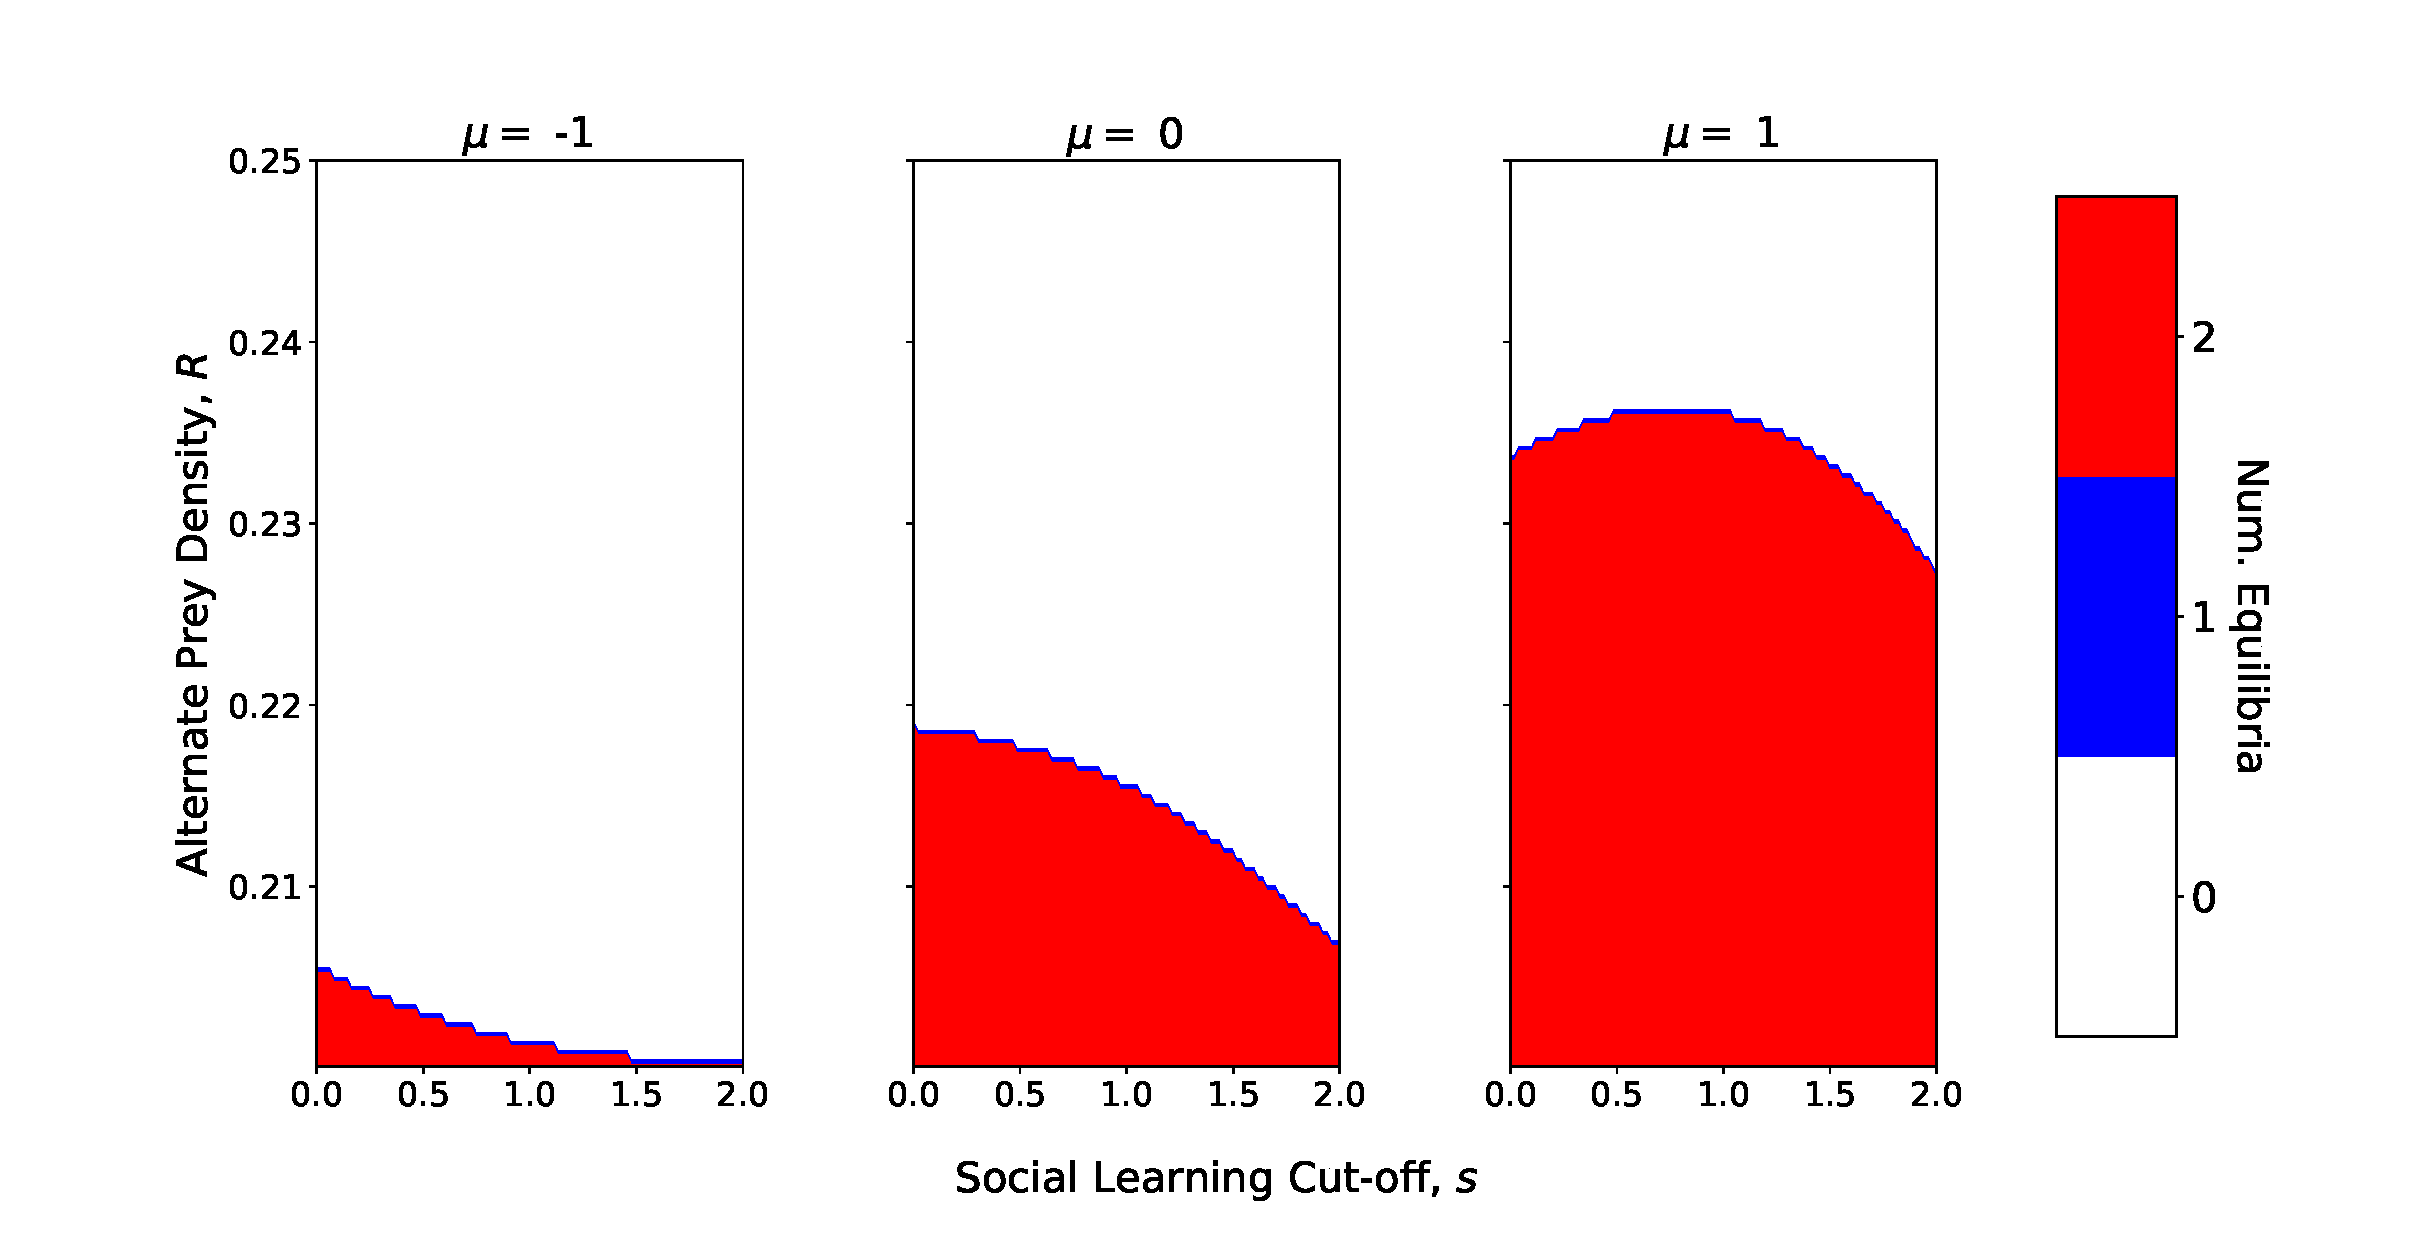
\includegraphics[width= 0.9\textwidth]{Figures_NoDelay/NumEquilibria_Rversuss_delta02_close.eps}
\caption{The number of nonzero $\hr$ equilibria for $\delta = 0.2$ and $R > \delta$, where the number of equilibria are indicated by colored regions, in relation to the social learning cut-off $s$ (x-axis) and alternate prey density $R$ for, from left to right, $\mu = -1,0,1$. We show only $R$ values for which $R < 0.25$ because for $R > 0.25$, there are no nonzero $\hr$ equilibria. }
\label{NoDelay_NumEq_close}
\end{center}
\end{figure}

\begin{figure}[htbp]
\begin{center}
\includegraphics[width= 0.9\textwidth]{Figures_NoDelay/Trajectories_R01_delta02_beta005_muNeg05_s1time.jpg}
\caption{Trajectories of the predator population size $N_p$ (blue), relative population density, $r$ of CP (red), and frequency $u_r$ of predators on CP (purple) with respect to time (in generations).  The parameters are: $R = 0.1, \delta = 0.2, \beta = 0.05, \mu = -0.5,$ and $s = 1$.The left y-axis is the number of individuals in the predator population, and the right y-axes are frequencies ($u_r$ or $r$), from 0 to 1. }
\label{NoDelay_traj1_time}
\end{center}
\end{figure}

\begin{figure}[htbp]
\begin{center}
\includegraphics[width= 0.9\textwidth]{Figures_NoDelay/Trajectories_R01_delta02_beta005_muPos05_s0time.jpg}
\caption{Trajectories of the predator population size $N_p$ (blue), relative population density, $r$ of CP (red), and frequency $u_r$ of predators on CP (purple) with respect to time (in generations). The parameters are: $R = 0.1, \delta = 0.2, \beta = 0.05, \mu = 0.5,$ and $s = 0$. The left y-axis is the number of individuals in the predator population, and the right y-axes are frequencies ($u_r$ or $r$), from 0 to 1. }
\label{NoDelay_traj1_time}
\end{center}
\end{figure}


\begin{figure}[htbp]
\begin{center}
\includegraphics[width= 0.9\textwidth]{Figures_NoDelay//Trajectories_R01_delta02_beta01.jpg}
\caption{Trajectories of the predator population size $N_p$, relative population density, $r$ of CP, and frequency $u_r$ of predators on CP, indicated by the y-axis, x-axis, and line colors, respectively, for 500 time steps. Arrows indicate the direction of the trajectory. Nonzero resource equilibria are indicated by stars, which are colored according to their $\hu_r$ values. For all four figures, $R = 0.1$, $\delta = 0.2$, and $\beta = 0.1$. For the top row of figures, the mean information quality is $\mu = -0.5$ and for the bottom row it is $\mu = 0.5$. For the figures on the left, there is no social learning i.e. $s = 0$, and for the figures on the right, the social learning cut-off is $s = 1$. All trajectories either end at the $\hr = \hN_p = 0$ equilibrium or the polymorphic equilibrium in which $\hN_p, \hr > 0$. The equilibria with at least one population going extinct (not marked with a star) are $\hr = \hN_p = 0$ and $\hN_p = 0$, $\hr = 1$. The magnitudes of the $J^*$ eigenvalues of the polymorphic equilibria, as calculated by \eqref{Jstar_evals}, are all less than one for each plot, indicating internal stability.}
\label{NoDelay_traj1}
\end{center}
\end{figure}

\begin{figure}[htb]
\centering
 \begin{subfigure}[b]{.4\textwidth}
	\centering
	\caption{$R = 0.1, \delta=0.5$}
	\includegraphics[width=0.95\textwidth]{Figures_NoDelay/Result3_1_R01_D05.jpg}
	\label{fig:result3_1a}
 \end{subfigure}
  \begin{subfigure}[b]{.4\textwidth}
	\centering
	\caption{$R=0.3, \delta=0.5$}
	\includegraphics[width=0.95\textwidth]{Figures_NoDelay/Result3_1_R03_D05.jpg}
	\label{fig:result3_1b}
 \end{subfigure}
 \newline
  \begin{subfigure}[b]{.4\textwidth}
	\centering
	\caption{$R=0.1, \delta=0.2$}
	\includegraphics[width=0.95\textwidth]{Figures_NoDelay/Result3_1_R01_D02.jpg}
	\label{fig:result3_1c}
 \end{subfigure}
   \begin{subfigure}[b]{.4\textwidth}
	\centering
	\caption{$R=0.6, \delta=0.8$}
	\includegraphics[width=0.95\textwidth]{Figures_NoDelay/Result3_1_R06_D08.jpg}
	\label{fig:result3_1d}
 \end{subfigure}
 \caption{Plots of Result \ref{Result_eq_Rlessthandelta}. Regions for which there is an equilibrium if $R < \delta$, i.e. consuming the alternate resource alone does not make up for the predator's death rate. }
  \label{fig:result3_1}
\end{figure}
% IN GENERAL SEEING THAT LOW PC--> NO EQUILIBRIA

\begin{figure}[htbp]
\begin{center}
\includegraphics[width=0.9\textwidth]{Figures_NoDelay//N_vs_s_R1delta3.jpg}
\caption{Equilibrium population size (vertical axis; $\hN_p$) versus social learning cut-off (horizontal axis; $s$) for $\mu = 0, \beta = 0.05$ (red line), $\mu = -0.5, \beta = 0.05$ (blue line), $\mu = 0, \beta = 0.02$ (red dots), $\mu = -0.5, \beta = 0.2$ (blue dots). Here $R = 0.1$ and $\delta = 0.3$}
\label{N_vs_s_R1delta3}
\end{center}
\end{figure}

\begin{figure}[htbp]
\begin{center}
\includegraphics[width=0.9\textwidth]{Figures_NoDelay//N_vs_s_R2delta3.jpg}
\caption{Like Fig. \ref{N_vs_s_R1delta3}, but $R - 0.2$ and $\delta = 0.3$. \red{Will fill in caption}}
\label{N_vs_s_R2delta3}
\end{center}
\end{figure}

\break

\begin{figure}[htbp]
\begin{center}
\includegraphics[width=0.9\textwidth]{Figures_NoDelay//Optimals_RlessthanDelta.jpg}
\caption{The value of $s$, called $s^*$ (vertical axis), which maximizes the predator population size at equilibrium, $\hN_p$, relative to mean environmental information quality $\mu$ (horizontal axis).}
\label{optimal_s_nodelay_RlessthanD}
\end{center}
\end{figure}

\begin{figure}[htbp]
\begin{center}
\includegraphics[width=0.9\textwidth]{Figures_NoDelay//Optimals_RlessthanDelta_muNeg025.jpg}
\caption{The value of $s$, called $s*$ (vertical axis), which maximizes the predator population size at equilibrium, $\hN_p$ relative to the frequency of AP, $R$ (horizontal axis) for mean environmental information quality $\mu = -0.25$.}
\label{optimal_s_nodelay_RlessthanD_R}
\end{center}
\end{figure}


%
%\begin{figure}[htbp]
%\begin{center}
%\includegraphics[width= 0.9\textwidth]{Figures_NoDelay//Trajectories_R01_delta02_beta005.jpg}
%\caption{Trajectories of the predator population size $N_p$, relative population density,$r$ of CP, and frequency $u_r$ of predators on CP, indicated by the y-axis, x-axis, and line colors, respectively, for 500 time steps. For all four figures, $R = 0.1$, $\delta = 0.2$, and $\beta = 0.05$. For the top row of figures, the mean information quality is $\mu = -0.5$ and for the bottom row it is $\mu = 0.5$. For the figures on the left, there is no social learning i.e. $s = 0$, and for the figures on the right, the social learning cut=off is $s = 1$. Nonzero resource equilibria are indicated by stars, which are colored according to their $\hu_r$ values. }
%\label{NoDelay_traj2}
%\end{center}
%\end{figure}
%
%\begin{figure}[htbp]
%\begin{center}
%\includegraphics[width= 0.9\textwidth]{Figures_NoDelay//Trajectories_R01_delta02_beta0025.jpg}
%\caption{Trajectories of the predator population size $N_p$, relative population density,$r$ of CP, and frequency $u_r$ of predators on CP, indicated by the y-axis, x-axis, and line colors, respectively, for 500 time steps. For all four figures, $R = 0.1$, $\delta = 0.2$, and $\beta = 0.025$. For the top row of figures, the mean information quality is $\mu = -0.5$ and for the bottom row it is $\mu = 0.5$. For the figures on the left, there is no social learning i.e. $s = 0$, and for the figures on the right, the social learning cut-off is $s = 1$. Nonzero resource equilibria are indicated by stars, which are colored according to their $\hu_r$ values. }
%\label{NoDelay_traj2}
%\end{center}
%\end{figure}
%
%\begin{figure}[htbp]
%\begin{center}
%\includegraphics[width= 0.9\textwidth]{Figures_NoDelay//Trajectories_R021_delta02_beta0025.jpg}
%\caption{Trajectories of the predator population size $N_p$, relative population density,$r$ of CP, and frequency $u_r$ of predators on CP, indicated by the y-axis, x-axis, and line colors, respectively, for 500 time steps. For all four figures, $R = 0.21$, $\delta = 0.2$, and $\beta = 0.025$. For the top row of figures, the mean information quality is $\mu = -0.5$ and for the bottom row it is $\mu = 0.5$. For the figures on the left, there is no social learning i.e. $s = 0$, and for the figures on the right, the social learning cut-off is $s = 1$. Nonzero resource equilibria are indicated by stars, which are colored according to their $\hu_r$ values. On the top row, the resource equilibria are $\hat{r} = .122, .056$ on the left and there are no equilibria on the right.  On the bottom row, the resource equilibria are $\hr = .179, .017$ on the left and $\hr = .183,.018$ on the right. Each trajectory in the top right plot has $N \to \infty$, and $r \to 0$. }
%\label{NoDelay_traj3}
%\end{center}
%\end{figure}
%
%
%
%\begin{figure}[htbp]
%\begin{center}
%\includegraphics[width= 0.9\textwidth]{Figures_NoDelay//Trajectories_R04_delta02_beta0025t10.jpg}
%\caption{Trajectories of the predator population size $N_p$, relative population density,$r$ of CP, and frequency $u_r$ of predators on CP, indicated by the y-axis, x-axis, and line colors, respectively, for 10 time steps. For all four figures, $R = 0.4$, $\delta = 0.2$, and $\beta = 0.025$. For the top row of figures, the mean information quality is $\mu = -0.5$ and for the bottom row it is $\mu = 0.5$. For the figures on the left, there is no social learning i.e. $s = 0$, and for the figures on the right, the social learning cut-off is $s = 1$. There are no nonzero resource equilibria, and instead $r \to 0$ and $N \to \infty$ (not shown). }
%\label{NoDelay_traj4}
%\end{center}
%\end{figure}

%\clearpage
%Page of results
%\begin{lemma} \label{Result_L_delta}
%If $\hN_p > 0$ at equilibrium and $R \neq \hr$, then
%\begin{equation} \label{delta_eq}
%L_u(\hu_r,\hr) = \frac{\delta-R}{\hr-R}.
%\end{equation}
%\end{lemma}
%
%
%\begin{lemma}
%If $R < \delta$, then there is one nonzero $\hu_r, \hr, \hN_p$ equilibrium if $\beta > 0$ and
%\begin{equation} \label{exists_eq_Rlessthan}
%\pc(1-R) + (\delta-R)(1+R) \lrp{ \frac{2K}{1+\delta} -1 } >0.
%\end{equation}
%\end{lemma}
%
%\begin{lemma}
%If $R > \delta$, then there exist two equilibria with $\hr > 0$ provided $Q_r''(r) > 0$, $-\delta Q_r''(r) < Q_r'(0)< 0$, and
%\begin{equation}
%(Q_r'(0))^2 - 2 Q_r''(r) Q_r(0) > 0.
%\end{equation}
% Otherwise, no $\hr >0$ equilibria exist. 
%\end{lemma}
%
%
%\begin{lemma}
%If $\hr = 0$ then $\hu_r = 0$, assuming $\pc > 0$, and if $R < \delta$, then $\hN_p = 0$.
%\end{lemma}
%
%\begin{lemma}
%If $\hN_p= 0$ and $\hr = 1$, then there is one possible equilibrium frequency $\hu_r>0$ of predators hunting the CP.
%\end{lemma}
%
%% E0, no delay
%\begin{lemma} \label{result_E0_nodelay}
%E0 is only stable along the nullcline $r = 0$ if $R < \delta$. Any point near the nullcline $r = 0$ will go to the nullcline if $R < \delta$, $R > - \frac{1-K}{1-2K u_r}$, and $1 - \beta N_p K u_r < 0$.
%\end{lemma}
%
%%% E1, no delay
%\begin{lemma} \label{E1_nodelay}
%Without a time delay, E1 is stable if 
%\begin{equation}
%R-\delta + (1-R) L(\hu_r,1) < 0
%\end{equation}
% and 
%\begin{equation}
%2K(1 - \hu_r(1-R)) < 1 + R + (1-R)\frac{\pc}{1+R}
%\end{equation}
%where $\hu_r$ is the larger root of $\eqref{E1_u}$.
%\end{lemma}
%
%
%Time Delay Stability Results:
%%% Delay, E0
%\begin{lemma}
%Result \ref{result_E0_nodelay} holds when there is a delay, i.e. E0 is unstable except along the $r = 0$ nullcline.
%\end{lemma}
%
%\begin{lemma}
%When there is a time delay, E1 is unstable under the same conditions as in the situation with no time delay (Result \ref{E1_nodelay}).
%\end{lemma}
%
%Irrespective of time delay:
%\begin{lemma}
%The resource depletion constant $\beta$ does not affect the social-learning cut-off $s^*$ that maximizes $\hN_p$ for any combination of the parameters $\mu, \delta, R$.
%\end{lemma}
%
%\begin{lemma}
%If $s = 0$, i.e. all predators are individual learners, then social learning evolves if $R < \delta$.
%\end{lemma}


\end{document}  